\documentclass{article}
\usepackage{booktabs}
\usepackage{amsmath}
\usepackage{amssymb}
\usepackage{geometry}
\usepackage{bm}
\usepackage{float}

\usepackage{xcolor}
\usepackage{subfig}
\usepackage{graphicx}
\usepackage{amsfonts}
\usepackage{multicol}
\usepackage{minted}
\usepackage{enumerate}

%[colorlinks,linkcolor=red,anchorcolor=blue,citecolor=green]
\usepackage[colorlinks, citecolor=red, linkcolor=blue]{hyperref}

%\setmainfont{CMU Serif}
%\usepackage{supertabular}
%\usepackage[font=normalsize]{caption}
%\usepackage{float}
%\usepackage{tikz}
%\usetikzlibrary{positioning,calc,decorations.pathreplacing}
%\usetikzlibrary{arrows,chains,scopes,graphs}
%\usepackage{minted}

\newcommand{\dg}{^{\circ}\mathrm{C}}
\newcommand{\rad}{\mathrm{rad}}
\newcommand{\ii}{\mathrm{i}}
\renewcommand{\d}{\mathrm{d}}
\newcommand{\e}{\mathrm{e}}

\setlength{\abovecaptionskip}{0.05cm}
\setlength{\belowcaptionskip}{0.05cm}

\title{Numerical Model of Calcium Valence Electrons}
\author{Jun Wang}
\date{Dec. 20, 2018}

\begin{document}
\maketitle
\section{Overview}
This \href{https://github.com/congzlwag/CaAtomSpec}{project} is building a quantum mechanical model of the two valence electrons in a Calcium atom. The purpose is to obtain full knowledge of states \textsf{[Ar]}$nln'l'~{}^{2S+1} L_J$, including
\begin{itemize}
\item Stark shift of a high Rydberg state
\item Linewidth of a high Rydberg state
\item Energy difference between states of interest
\end{itemize}

The Hilbert space of the two-particle system $\mathcal H$ is the antisymmetrized direct product of two single-body Hilbert space $\mathcal A (\mathcal H_1\otimes \mathcal H_1)$. The total Hamiltonian is 
\begin{equation}
H = \sum_{k=1,2} h_0(k) + V + H_\mathrm{SOC},
\end{equation}
%h &= h_0 +\xi(r)\bm{s}\cdot\bm{l},\\
\begin{gather}
V = \frac{e^2}{4\pi\epsilon_0 |\bm{r}_1-\bm{r}_2|},\\
h_0 = \frac{-\hbar^2}{2\mu}\bm{\nabla}^2 + U(r) = \frac{-\hbar^2}{2\mu r^2}\partial_r r^2\partial_r + \frac{\bm{l}^2}{2\mu r^2} + U(r),\\
H_\mathrm{SOC} = \sum_{k=1,2}\xi(r_k)\bm{s}_k\cdot\bm{l}_k + \sum_{k_1\neq k_2}\eta(r_{k_1},r_{k_2},|\bm{r}_1-\bm{r}_2|)\bm{s}_{k_1}\cdot\bm{l}_{k_2}~,
\end{gather}
where $U(r)$ is the model potential produced by the Ca${}^{2+}$ core for a single electron, depending only on the radial distance. $\xi(r) = \frac{1}{2m_e^2c^2}\frac{\mathrm{d}U}{r\mathrm{d}r}$, and as for the inter-electron spin-orbit coupling coefficient $\eta(r_1,r_2,|\bm{r}_1-\bm{r}_2|)$, I do not have its specific form but supposedly it depends on their distance to the center and their relative distance.

\subsection{Units and Notation Conventions}

The numerical implementation is in \href{https://en.wikipedia.org/wiki/Atomic_units#cite_note-Hartree28-1}{(Hatree) Atomic Units}, which is elaborated in Tab. \ref{tab:units} .
\begin{table}[htbp]
\centering
\caption{Useful expressions and values in (Hatree) Atomic Units, extracted from Ref. \cite{au:wiki} .}\label{tab:units}
\begin{tabular}{c|c|c|c}
\hline\hline
Dimension	&Expression(s)	&Value in SI	&Value in other units \\ \hline
Length		&$a_0 = \frac{4\pi\epsilon_0 \hbar^2}{m_e e^2}$	&$0.5292\mathrm{\AA}$	& \\ \hline
Angular momentum	&$\hbar$	&$1.055\times 10^{-34}$J$\cdot$s	&\\ \hline
Mass	& $m_e$	& $9.109\times 10^{-31}$kg	&	\\ \hline
Energy	&$E_H= \frac{m_e e^4}{(4\pi\epsilon_0\hbar)^2} = \frac{\hbar^2}{m_ea_0^2} = \alpha^2 m_ec^2$	&	$4.360\times 10^{-18}$J	&$27.21$eV \\ \hline
Frequecy	& $E_H/\hbar$	&	$4.134\times 10^{16}$Hz	&\\ \hline
Velocity	& $E_Ha_0/\hbar = \frac{e^2}{4\pi\epsilon_0\hbar} = \alpha c$ 		&$2.188\times 10^{6}$m/s 	& $7.297\times 10^{-3}$c\\ \hline
\end{tabular}
\end{table}
In this unit system, the terms in the Hamiltonian are
\begin{gather}
%H = \sum_{k=1,2} h_0(k) + V +H_\mathrm{SOC},\\
%h = h_0 +\xi(r)\bm{s}\cdot\bm{l},\\
V = \frac{1}{|\bm{r}_1-\bm{r}_2|},\\
h_0 = \frac{-1}{2\mu r^2}\partial_r r^2\partial_r + \frac{\bm{l}^2}{2\mu r^2} + U(r),\\
\xi(r) = \frac{\alpha^2}{2}\frac{\mathrm{d}U}{r\mathrm{d}r},
\end{gather}
where $\alpha =\frac{e^2}{4\pi\epsilon_0\hbar c}$ is the fine-structure constant. 
$U(+\infty) = 0$ indicates that the reference point of the total energy corresponds to the state where both the valence electrons are ionized, i.e. Ca III (${}^{1}\mathrm{S}_0$) \cite{SC85}.

Aside from the (Hatree) Atomic Unit, there are some other conventions about notation:
\begin{itemize}
\item $\phi$ is an orbital wavefunction, while $\psi$ is a total wavefunction taking 2 by 1 column vector values;
\item Some quantities are capitalized to stress that they are of two-particle system, distinguished from their single-particle counterparts, e.g. $E,\bm{L},\Phi, \Psi$ from $\epsilon,\bm{l},\phi,\psi$.
\item $\mathcal P_{12}$ refers to the transposition of the identities of the two electrons. Note that for a total wavefunction $\Psi$ it transposes the tensor indices besides swaping $\bm{r}_1,\bm{r}_2$;
\item $\mathcal A$ is the normed antisymmetrization operator. For any (orbital or total) two-body wavefunction $\Psi$
\begin{gather}
\left(\mathcal{A}\Psi\right) \equiv (\Psi - \mathcal P_{12}\Psi)/||\Psi - \mathcal P_{12}\Psi||_2\label{eq:defA}\\
||\Psi||_2 \equiv \sqrt{\int\d^3\bm{r}_1\d^3\bm{r}_2\Psi(\bm{r}_1,\bm{r}_2)^\dagger\Psi(\bm{r}_1,\bm{r}_2)}
\end{gather}
\end{itemize}

\subsection{Implementation}

It is straightforward to verify that $0=[V, \bm{L}]=[V, \bm{S}]=[V,\bm{J}] $, and $\forall k_1,k_2\in\{1,2\}, \bm{s}_{k_1}\cdot\bm{l}_{k_2}$ commutes with $\bm{L}^2,\bm{S}^2$ and $\bm{J}$. Therefore $H, \bm{L}^2, \bm{S}^2, \bm{J}^2, J_z$ comprise a commutable set of conservatives. Even the orbit-orbit coupling $\bm{l}_1\cdot\bm{l}_2$ and spin-spin coupling $\bm{s}_1\cdot\bm{s}_2$ terms, which are neglected at the very beginning, commute with $\bm{L}^2, \bm{S}^2, \bm{J}^2, J_z$. As a result, an atom (and atomic ion) state can be marked by quantum numbers $L,S,J,M_J$, and $M_J$ is usually left out when describing a level due to degeneracy. 

In lighter elements, the deviation of an energy level from the product state energy is dominated by electrostatic interactions $V$, so $LS$ coupling is adopted. However $\bm{L}^2, \bm{S}^2, \bm{J}^2, J_z$ is not a complete set, so the eigenstate is a superposition of different electron configurations in the eigen subspace marked by $L,S,J,M_J$, and the state marked by $(n_1,l_1,n_2,l_2), L,S,J,M_J$ is not an eigenstate of $\bm{l}_1^2, \bm{l}_2^2$ but the eigenstate that overlaps the most with the electron configuration $(n_1,l_1,n_2,l_2)$. The workflow for obtaining it is
\begin{enumerate}
\item Solve all single electron states from $h_0 \psi = \epsilon \psi$;
\item In an eigen subspace marked by $L,S,J,M_J$:
\begin{enumerate}[(1)]
\item Compute the matrix elements of $V$ and $H_\mathrm{SOC}$;
\item Choose a set of electron configurations that are relevant to the perturbation of the state of interest, as the computational basis;
\item Construct the matrix of $H$ and diagonalize;
\item Pick the eigenvector that overlaps the most with the electron configuration of interest.
\end{enumerate}
\end{enumerate}
%\begin{equation}
%H = \sum_{k=1,2} h_0(k) + \frac{1}{|\bm{r}_1-\bm{r}_2|} + \sum_{k=1,2}\xi(r_k)\bm{s}_k\cdot\bm{l}_k
%\end{equation}

The codes and references are available on \href{https://github.com/congzlwag/CaAtomSpec}{Github}.
\section{Single Particle States}
\subsection{Model Potential $U(r)$}

The Klapisch form is adopted for the model potential $U(r)$, including a screening term and a polarization term
\begin{equation}
U(r) \equiv \frac{-1}{r}(2+18\e^{-a_1^{(l)} r} - r(a_3^{(l)} + a_4^{(l)}r)\e^{-a_2^{(l)}r}) - \frac{\alpha_d}{2r^4}(1-\e^{-(r/r_c^{(l)})^6}),
\end{equation}
and the parameters $a_1, a_2, a_3, a_4, r_c$ are $l$-dependent. The dipole polarizability of the Ca${}^{2+}$ core $\alpha_d$ is not. Table \ref{tab:Aymar1991} lists an optimized set that is restricted to $\alpha_d=3.5, a_4=0$,
\begin{table}[htbp]
\caption{4-parameter model potential of Klapisch form optimized by \cite{Aymar_1991}} \label{tab:Aymar1991}
\centering
\begin{tabular}{r|cccc}
\hline\hline
$l$ & $a_1$ & $a_2$ &$a_3$ &		$r_c$ \\ \hline
0 & 4.0099	& 2.1315 &	-13.023 &	1.6352	\\ \hline
1 & 4.2056	& 2.0186	&	-12.658 & 1.5177 	\\ \hline
2 & 3.5058	& 2.2648	& 	-12.399 & 1.6187	\\ \hline
$\geq$ 3 & 3.7741	& 3.1848	&-13.232&0.7150	\\ \hline
\end{tabular}
\end{table}
A comprehensive list of $\alpha_d$ values could be found in \cite{PhysRevA.88.062504}, including an experimental value \cite{UOpik_1967} $\alpha_d=3.26$ and theoretical values centered around this one. Since \cite{Aymar_1991} cited nothing for its $\alpha_d=3.5$, optimization for $\alpha_d=3.26$ is potentially necessary. For now, just keep it in mind.

\subsection{Radial Equation}
Since $h_0$ has nothing to do with spin and $0=[h_0,\bm{l}^2]=[h_0,l_z]$, separating variables in $h_0 \psi = \epsilon \psi$, one sets
\begin{equation}
\psi_{n,l,m,m_s}(\bm{r}) = \phi_{n,l,m}(\bm{r})\chi(m_s) = \frac{u_{nl}(r)}{r} Y_{lm}(\bm{r}/r) \chi(m_s),
\end{equation}
where $u_{nl}$ is the radial function to be solved, and
\begin{gather}
Y_{lm}(\theta,\varphi) = \sqrt{\frac{(2l+1)(l-m)!}{4\pi (l+m)!}}\e^{\ii m \varphi} P_l^m(\cos\theta);\\
\chi(m_s) = (\delta_{m_s,1/2}, \delta_{m_s,-1/2})^T .
\end{gather}
From the single particle Schr\"{o}dinger equation, one obtains the radial equation:
\begin{align}
\epsilon_{n,l} \frac{u_{nl}(r)}{r} &= \left(\frac{-1}{2\mu r^2}\partial_r r^2\partial_r + \frac{l(l+1)}{2\mu r^2} + U(r)\right) \frac{u_{nl}(r)}{r}, \\
\text{ i.e. }\epsilon_{n,l} u_{nl}(r) &= \left(\frac{-1}{2\mu}\frac{\d^2}{\d r^2}+ \frac{l(l+1)}{2\mu r^2} + U(r)\right) u_{nl}(r),\\
\text{ i.e. }\frac{\d^2u_{nl}(r)}{\d r^2}&+\gamma(r)u_{nl}(r) = 0\label{eq:radial-main},~~\gamma(r) = 2\mu(\epsilon_{n,l}-U(r))-\frac{l(l+1)}{r^2} ,
\end{align}
which also indicates that $u_{nl}(r)\in\mathbb{R}$ .

In order for better convergence properties, transform eq.(\ref{eq:radial-main}) into the differential equation of variable $y(x) = x^{-1/2}u(x^2), x = \sqrt{r}$, 
\begin{equation}
\frac{\d^2y}{\d x^2} + g(x) y(x) = 0,~~g(x) = 4x^2\gamma(x^2) -\frac{3}{4x^2}\label{eq:defg}
\end{equation}
Discretizing with \href{https://en.wikipedia.org/wiki/Numerov\%27s_method}{Numerov difference form} and gridding $x$ with even step length $h$
\begin{align}
\frac{y_{k-1}-2y_k+y_{k+1}}{h^2} + \frac{1}{12}g_{k-1}y_{k-1} + \frac{10}{12}g_{k}y_{k} +  \frac{1}{12}g_{k+1}y_{k+1}  &= 0 \\
\text{i.e.} ~~(1+\frac{h^2}{12}g_{k-1})y_{k-1} + (-2 +\frac{10 h^2}{12}g_k)y_k + (1+\frac{h^2}{12}g_{k+1})y_{k+1} &= 0\label{eq:radial-diffed}
\end{align}
Recall the definitions of $g(x), \gamma(r)$ in Eq.(\ref{eq:defg})(\ref{eq:radial-main}), and define $W(x)$, one obtains
\begin{equation}
g(x) = 8\mu x^2\epsilon_{n,l} - W(x),\quad W(x)= 8\mu U(x^2)+\frac{4(l+1/4)(l+3/4)}{ x^2}
\end{equation}

I wrote a python module \mintinline{python}{numerov} in C++ to either integrate the radial function or solve the eigenequation of the radial function. For Mac OS X, the .so file is ready in \mintinline{bash}{./Numerov}; For other Unix systems, one can simply run \mintinline{bash}{./pyCppbuild} in the directory of \mintinline{bash}{./Numerov} to obtain the corresponding .so file. To use this module, one can either copy this .so file to the current working path or claim \mintinline{python}{sys.path.append("[path of the Dev folder]/Numerov")} in the python scripts.

The module also supports solving the radial function in the Schr\"{o}dinger equation with SOC term:
\begin{equation*}
h \left\{\frac{u_{nlj}(r)}{r}\sum_{m}\langle l,m_l,\frac{1}{2},m-m_l|j,m\rangle Y_{lm_l}(\frac{\bm{r}}{r})\chi(m-m_l)\rangle\right\} = \epsilon_{n,l,j} \sum_{m_l}\langle l,m_l,\frac{1}{2},m-m_l|j,m\rangle Y_{lm_l}(\frac{\bm{r}}{r})\chi(m-m_l)
\end{equation*}
Please refer to the documentation of the functions \mintinline{python}{numerov.integrate} and \mintinline{python}{numerov.eigensolve}.

\subsubsection{Integration}
The integration function \mintinline{python}{numerov.integrate} simply integrates inwards according to eq.(\ref{eq:radial-diffed}). Because the error of the model potential is smaller outside the Ca$^{2+}$ region, integrating inwards is more credible than outwards.
\begin{equation}
y_{k-1} = \left(1+\frac{h^2}{12}g_{k-1}\right)^{-1} \left((2 -\frac{10 h^2}{12}g_k)y_k - (1+\frac{h^2}{12}g_{k+1})y_{k+1}\right)
\end{equation}

\subsubsection{Solving eigen equation}
In Eq.(\ref{eq:radial-diffed}), moving all the $\epsilon$ terms to the r.h.s
\begin{equation}
(1-\frac{h^2}{12}W_{k-1})y_{k-1} + (-2-\frac{10h^2}{12}W_k)y_k + (1-\frac{h^2}{12}W_{k+1})y_{k+1} = -\frac{2\mu}{3}\epsilon(r_{k-1}y_{k-1} + r_ky_k + r_{k+1}y_{k+1}),\label{eq:radial-eig}
\end{equation}
it is now in the form $A\cdot x =\lambda M\cdot x$, where both $A,M$ are tri-diagonal real matrices and thus can be easily LU decomposed. Avoiding ill-conditioned $M$, both sides of Eq.(\ref{eq:radial-eig}) are divided by $r_k$ before applying the subroutine that solves $\lambda, x$ from $A\cdot x =\lambda M\cdot x$. For details about this subroutine, please refer to App. \ref{app:Ax=lMx}.

\subsection{Assessment of model parameters, in terms of CaII spectra}
In order to assess the model parameters qualitatively, one should look into the mismatch between the solved eigenenergies and the experimental values. What we need in the following computation is the eigenbasis of $h_0$, while the experimental values in Ref. \cite{SC85} are with fine structure. From the fine structure split
\begin{equation}
\langle\bm{l}\cdot\bm{s}\rangle = \left\{
\begin{array}{ll}
\frac l2 &\text{if }j=l+\frac 12\\
\frac{-(l+1)}{2} &\text{if }j=l-\frac{1}{2},
\end{array}\right.
\end{equation}
one obtains
\begin{equation}
\epsilon_{n,l} = \left\{
\begin{array}{ll}
\epsilon_{n,0,1/2} & \text{if }l=0,\\
\frac{l+1}{2l+1}\epsilon_{n,l,l+1/2} + \frac{l}{2l+1}\epsilon_{n,l,l-1/2} & \text{if }l>0 ,
\end{array}\right.
\end{equation}
\mintinline{bash}{./specs/CaII_ebar.npz} includes these averaged $\epsilon_{n,l}$ processed from $\epsilon_{n,l,j}$ data in \mintinline{bash}{./specs/CaII.npz} . With the model parameters in Tab. \ref{tab:Aymar1991}, the relative errors of eigenenergies, with respect to the experimental $\epsilon_{n,l}$ data, square root meaned over different $n$ for the same $l$, are no larger than $5\times 10^{-4}$.

\subsection{Extrapolation with quantum defects}
Either integrate or solve the eigen equation for radial function $u_{nl}$ or single-particle wavefunction $\psi_{n,l,m,m_s}$, at least an approximate value of energy $\epsilon_{n,l}$ is necessary. The experimental values \cite{SC85}, however, are limited after all. In order for $\psi_{n,l,m,m_s}$ of arbitrary $n,l$, I extrapolated the experimental $\epsilon_{n,l}$ with an $l$-dependent quantum defect:
\begin{equation}
\epsilon_{n,l} = \frac{-1}{2(n-\delta_l)^2} .
\end{equation}
\begin{figure}
\centering
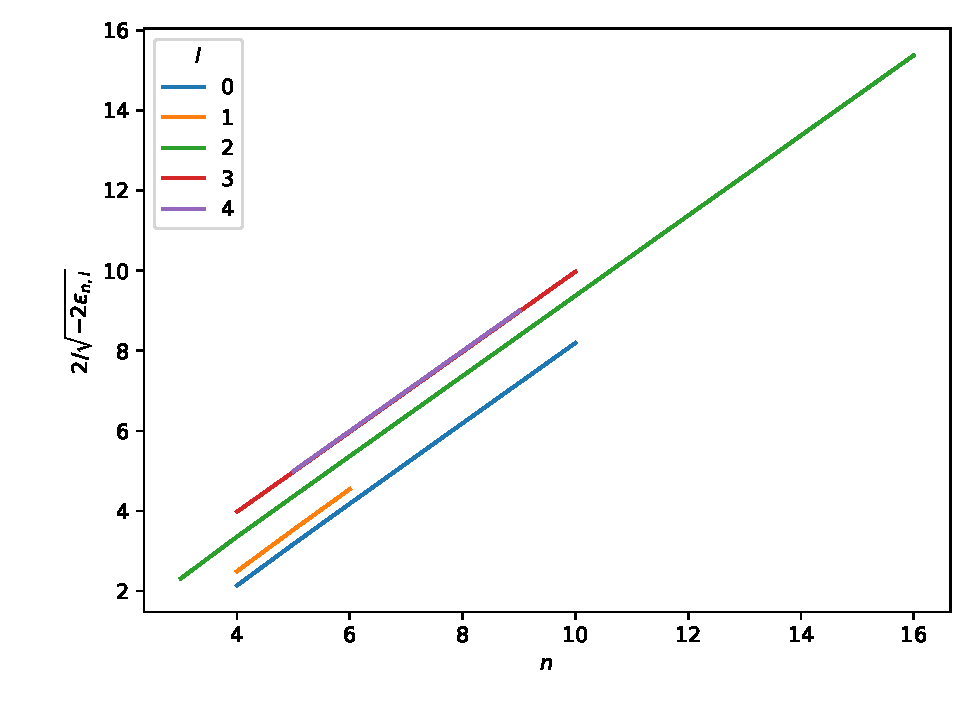
\includegraphics[width=0.7\linewidth]{../Dev/QD.pdf}
\caption{Fitting quantum defect parameters from experimental values of CaII energies.}\label{fig:QD}
\end{figure}
The linear dependence of $2/\sqrt{-2\epsilon_{n,l}}$ on $n$ is quite obvious in Fig.\ref{fig:QD} , namely, $\epsilon_{n,l} = \frac{-1}{2(\alpha_ln-\delta_l)^2}$ with $\alpha_l, \delta_l$ being the fitting parameters.
The fitting results are stored in \mintinline{bash}{./specs/ebar_quant_defect.pickle} , and unsurprisingly all $\alpha_l$ are all close to unity.  Note that $l=3,4$ are close enough to each other, I assume $l>4$ has the same quantum defect as $l=4$.

Now for arbitrary $n,l$, one has the energy $\epsilon_{n,l}$, which is the experimental value if could be found or extrapolated otherwise. This is implemented in \mintinline{python}{request_energy} in \mintinline{bash}{./LS.py}, and the radial wavefunction $u_{nl}$ is subsequently obtained via Numerov integration, implemented in \mintinline{python}{request_ur} .

\section{Coupling to Two-Particle States}
%\subsection{Zero Order}
Now the single particle basis $\{\psi_{n,l,m,m_s} | n \geq 3; l<n,~l\geq 0 \text{ if } n>3 \text{ else } 2; |m|\leq l; m_s=\pm\frac{1}{2}\}$ is ready. The Hilbert space $\mathcal H$ can be spanned by the antisymmetrized direct products ${\mathcal{A}(\psi_{n1,l1,m1,m_s1}\otimes\psi_{n2,l2,m2,m_s2})}$, or any complete set of linear combination of them. By $LS$ coupling it means the basis $\mathcal B$ is structured as
\begin{align}
\mathcal B &\equiv \{\mathcal B_{L,S,J,M_J}|L\in\mathbb{N};S=0,1;J=|L-S|,\cdots,L+S; M_J = -J,\cdots,+J\}~,\\
\mathcal B_{L,S,J,M_J} &\equiv \{\mathcal A\tilde\Psi_{\gamma,L,S,J,M_J}|\gamma=(n_1,l_1,n_2,l_2)\text{ is compatible with }L,S\}~,
\end{align}
where
\begin{align}
\tilde\Psi_{\gamma,L,S,J,M_J}&\equiv\sum_{M_S}\langle L,M_J-M_S,S,M_S | J,M_J\rangle\Psi_{\gamma,L,M_J-M_S,S,M_S}~,\\
\Psi_{\gamma,L,M_L,S,M_S}(\bm{r}_1,\bm{r}_2) &\equiv \Phi_{\gamma,L,M_L}(\bm{r}_1,\bm{r}_2) X_{S,M_S}\\
\Phi_{(n_1,l_1,n_2,l_2),L,M_L}(\bm{r}_1,\bm{r}_2) &\equiv \sum_{m_1,m_2}\langle l_1m_1,l_2m_2 | LM_L\rangle \phi_{n_1,l_1,m_1}(\bm{r}_1) \phi_{n_2,l_2,m_2}(\bm{r}_2) \nonumber\\
&= \frac{u_{n_1l_1}(r_1)u_{n_2l_2}(r_2)}{r_1r_2}Y_{l_1,l_2,L,M_L}(\bm{\hat r}_1,\bm{\hat r}_2)\label{eq:Psi-orbit}~,
\end{align}
and $Y_{l_1,l_2,L,M_L}(\bm{\hat r}_1,\bm{\hat r}_2), X_{S,M_S}$ are the coupled two-body orbit wavefunction and spin state (a rank-$2$ tensor with both $2$-dimensional indices) respectively. By ``compatible" I mean (1) $l_1+l_2 \geq L \geq |l_1-l_2|$ and (2) non-zero after antisymmetrization.

Note that $\langle j_2m_2,j_1m_1 | JM\rangle = (-1)^{J-j_1-j_2}\langle j_1m_1,j_2m_2 | JM\rangle$, the transposition causes
\begin{gather}
\mathcal P_{12}X_{S,M_S} = (-1)^{S-1}X_{S,M_S},\\
\mathcal P_{12}Y_{l_1,l_2,L,M_L}(\bm{\hat r}_1,\bm{\hat r}_2)\equiv Y_{l_1,l_2,L,M_L}(\bm{\hat r}_2,\bm{\hat r}_1) = (-1)^{L-l_1-l_2}Y_{l_2,l_1,L,M_L}(\bm{\hat r}_1,\bm{\hat r}_2),
\end{gather}
which gives
\begin{align}
\mathcal P_{12}\Psi_{\gamma,L,S} &= (-1)^{S+L-1-l_1-l_2} \Psi_{(n_2,l_2,n_1,l_1),L,S} \label{eq:P12Psi}\\
&=\left\{
\begin{array}{ll}
(-1)^{S+L-1}\Psi_{\gamma,L,S} & \text{if }n_1=n_2, l_1=l_2 ,\\
\text{Linear independent from }\Psi_{\gamma,L,S} &\text{otherwise} ,
\end{array}\right.
\end{align}
where $\Psi_{\gamma,L,S}$ stands for a generic state in the eigen subspace marked by $\gamma, L,S$ whose special cases include $\tilde\Psi_{\gamma,L,S,J,M_J}$ and $\Psi_{\gamma,L,M_L,S,M_S}$. The normalization factor is thus
\begin{equation}
N_{\gamma,L,S} \equiv ||\Psi_{\gamma,L,S}-\mathcal P_{12} \Psi_{\gamma,L,S}||_2 = \left\{
\begin{array}{ll}
1+(-1)^{S+L-1} & \text{if }n_1=n_2, l_1=l_2 ,\\
\sqrt{2} &\text{otherwise} .
\end{array}\right.
\end{equation}

A routine that is frequently adopted when calculating the matrix elements of a scalar symmetric observable $O, \mathcal{P}_{12}O = O$ comes as follow:
\begin{align}
\langle \mathcal A\Psi' |O| \mathcal A\Psi\rangle &= \frac{2}{N'N}\left(\langle\Psi'|O|\Psi\rangle - \langle\Psi'|O|\mathcal P_{12}\Psi\rangle\right) \nonumber\\
&= \frac{2}{N'N}\left(\langle\Psi'|O|\Psi\rangle+(-1)^{S+L-l_1-l_2} \mathcal P(n_1\leftrightarrow n_2, l_1\leftrightarrow l_2)\{\langle\Psi'|O|\Psi\rangle\}\right),\label{eq:OO}
\end{align}
where $\mathcal P(n_1\leftrightarrow n_2, l_1\leftrightarrow l_2)$ swaps $n_1,l_1$ with $n_2,l_2$ in the sandwich, and $\Psi',\Psi$ are shorthands for $\Psi_{\gamma',L',S'}, \Psi_{\gamma,L,S}$.

\subsection{Matrix elements}\label{sec:mat-elements}
Because $\psi_{n,l,m,m_s}$ are degenerate over $m,m_s$, it is clear that
\begin{equation}
(h_0(1)+h_0(2))\mathcal A \Psi_{(n_1,l_1,n_2,l_2),L,S} = (\epsilon_{n_1,l_1} + \epsilon_{n_2,l_2}) \mathcal A \Psi_{(n_1,l_1,n_2,l_2),L,S}~.
\end{equation}

\subsubsection{Electronstatic interaction $V$}
Separating variables
\begin{equation}
V(\bm{r}_1,\bm{r}_2) = \sum_{l=0}^{+\infty}\frac{4\pi\min(r_1,r_2)^l}{(2l+1)\max(r_1,r_2)^{l+1}}\sum_{m=-l}^{l}Y_{lm}(\bm{\hat r}_1)Y_{lm}(\bm{\hat r}_2)^*~,
\end{equation}
one obtains
\begin{equation}
\langle \Phi_{\gamma',L,M_L} |V| \Phi_{\gamma,L,M_L}\rangle = \sum_{l=0}^{+\infty}\text{angulaV}(l,l'_1,l'_2,l_1,l_2;L,M_L) \text{radiaV}(l,u_{n'_1l'_1},u_{n'_2l'_2},u_{n_1l_1},u_{n_2l_2})
\end{equation}
%can be separated into the direct and the exchange parts
%\begin{equation}
%\langle \mathcal A\Psi_{\gamma',L,M_L,S,M_S} | V | \mathcal A\Psi_{\gamma, L,M_L,S,M_S} \rangle %&= \frac{1}{N_{\gamma'}N_\gamma} \langle\Psi_{\gamma'}(1,2)-\Psi_{\gamma'}(2,1)|V(\bm{r}_1,\bm{r}_2)|\Psi_\gamma(1,2)-\Psi_\gamma(2,1)\rangle\nonumber\\
%= \frac{2}{N_{\gamma'}N_\gamma} \langle\Psi_{\gamma'}(1,2)|V(\bm{r}_1,\bm{r}_2)\left(|\Psi_\gamma(1,2)\rangle-|\Psi_\gamma(2,1)\rangle\right)% =: \frac{2}{N_{\gamma'}N_\gamma} (\tilde V_{\mathrm{dr}} - \tilde V_\mathrm{ex})
%%\left(\frac{u_{n'_1l'_1}(r_1)u_{n'_2l'_2}(r_2)}{r_1r_2}Y_{l'_1,l'_2,L,M_L}(\bm{\hat r}_1,\bm{\hat r}_2)\right)^*
%% &= \int \d^3\bm{r}_1\int\d^3\bm{r}_2\Phi_{\gamma'}(\bm{r}_1,\bm{r}_2)^* \sum_{l=0}^{+\infty}M_l(r_1,r_2)\frac{4\pi}{2l+1}\sum_{m=-l}^{l}(-1)^mY_{l,-m}(\bm{\hat r}_2)Y_{l,m}(\bm{\hat r}_1) \left(\Phi_{\gamma}(\bm{r}_1,\bm{r}_2)-\Phi_\gamma(\bm{r}_2,\bm{r}_1)\right)
%\end{equation}
%To reduce spam, $L,M_L,S,M_S$ in subscripts are left out. Expanding $V(\bm{r}_1,\bm{r}_2)$ with the additional formula of spherical harmonics and defining:
defining
\begin{align}\label{eq:V-LS}
\text{angulaV}(l,l'_1,l'_2,l_1,l_2;L,M_L) &\equiv \sum_{m=-l}^l\int\d\Omega_1\int\d\Omega_2 Y_{l'_1,l'_2,L,M_L}(\bm{\hat r}_1,\bm{\hat r}_2)^*Y_{l,m}(\bm{\hat r}_2)^*Y_{l,m}(\bm{\hat r}_1)Y_{l_1,l_2,L,M_L}(\bm{\hat r}_1,\bm{\hat r}_2),\\
\text{radiaV}(l,u_{1'},u_{2'},u_{1},u_2) &\equiv \int_0^{+\infty}\d r_1\int_0^{+\infty}\d r_2 u_{1'}(r_1)u_{2'}(r_2)\frac{4\pi\min(r_1,r_2)^l}{(2l+1)\max(r_1,r_2)^{l+1}}u_{1}(r_1)u_{2}(r_2)~.
\end{align}
Further evaluation of $\text{angular}(l,l'_1,l'_2,l_1,l_2;L,M_L)$ into Wigner-3j symbols (See App. \ref{app:angulaV}) shows that $l\in [|l'_1-l_1|,l'_1+l_1]\cap[|l'_2-l_2|,l'_2+l_2]$ is necessary for its being non-zero, so the summation over $l$ in Eq. (\ref{eq:V-LS}) is finite. 

Moreover, $V$ is isotropic and has nothing to do with the spin. 
Therefore the degeneracy over $M_L, M_S$ is preserved in the representation of $V$. Namely, the $V$ matrix is independent of $M_L, M_S$. Thus I can compute it in the $M_L=L$ subspace for simplicity and denote 
\begin{equation}
\langle \gamma',L |V|\gamma,L\rangle \equiv \sum_{l=0}^{+\infty}\text{angulaV}(l,l'_1,l'_2,l_1,l_2;L,L) \text{radiaV}(l,u_{n'_1l'_1},u_{n'_2l'_2},u_{n_1l_1},u_{n_2l_2})~,
\end{equation}
and I have $\langle \tilde \Psi_{\gamma',L,S,J,M_J} |V| \tilde\Psi_{\gamma,L,S,J,M_J}\rangle=\langle \gamma',L|V|\gamma,L\rangle$ because $\{\tilde \Psi_{\gamma',L,S,J,M_J}|J,M_J\}$ is unitarily transformed from $\{\Psi_{\gamma,L,M_L,S,M_S}|M_L,M_S\}$.

Since $V$ is symmetric, one adopts Eq. (\ref{eq:OO}),
\begin{align}
&\langle \mathcal A\tilde\Psi_{\gamma',L,S,J,M_J} | V | \mathcal A\tilde\Psi_{\gamma,L,S,J,M_J} \rangle \nonumber\\
=& \frac{2}{N_{\gamma',L,S}N_{\gamma,L,S}} (\langle \gamma',L |V|(n_1,l_1,n_2,l_2),L\rangle +(-1)^{S+L-l_1-l_2}\langle \gamma',L |V|(n_2,l_2,n_1,l_1),L\rangle)\label{eq:V-final}
%=& \frac{2}{N_{\gamma',L,S}N_{\gamma,L,S}}\sum_{l=0}^{+\infty} \Big(\text{angulaV}(l,l'_1,l'_2,l_1,l_2;L,L) \text{radiaV}(l,u_{n'_1l'_1},u_{n'_2l'_2},u_{n_1l_1},u_{n_2l_2})\nonumber\\
%&+(-1)^{S+L-l_1-l_2}\text{angulaV}(l,l'_1,l'_2,l_2,l_1;L,L)\text{radiaV}(l,u_{n'_1l'_1},u_{n'_2l'_2},u_{n_2l_2},u_{n_1l_1})\Big) . 
\end{align}

\subsubsection{Spin-orbit coupling}
It is generally observed that $0= [\bm{s}_{k_1}\cdot\bm{l}_{k_2}, \bm{l}^2_{k_3}]~\forall k_1,k_2,k_3\in\{1,2\}$, which results in that $H_\mathrm{SOC}$ commutes with $\bm{l}_1^2,\bm{l}_2^2$ aside from $\bm{L}^2,\bm{S}^2,\bm{J}$. 
%Therefore
%\begin{itemize}
%\item $l_1,l_2,J,M_J$ are still good quantum numbers.
%\item $M_J$ degeneration is preserved.
%\end{itemize}
%In the eigen subspace marked by $L, S$, let's %omit the inter-electron spin-orbit term in $H_\mathrm{SOC}$ term,  consider $\sum_{k=1,2}\xi(r_k)\bm{s}_k\cdot\bm{l}_k$ for now. Since $[\bm l\cdot\bm s, j_\alpha] = 0,~\alpha=x,y,z$, $J,M_J$ are still good quantum numbers after perturbed by $H_\mathrm{SOC}$, so let's 
%transit to another basis spanned by
%\begin{gather}
%\Psi^\mathrm{LS}_{\gamma,L,S,J,M_J} =\sum_{\beta} c_{\beta}^{(\gamma)}\mathcal A\tilde\Psi_{\beta,L,S,J,M_J},\\
%\tilde\Psi_{\beta,L,S,J,M_J}\equiv\sum_{M_S}\langle L,M_J-M_S,S,M_S | J,M_J\rangle\Psi_{\beta,L,M_J-M_S,S,M_S}~,
%\end{gather}
%then it is clear that the representation of $H_\mathrm{SOC}$ is diagonal in the subspace marked by $\gamma,L,S$, namely $\{\Psi^\mathrm{LS}_{\gamma,L,S,J,M_J} | J=|L-S|,\cdots,L+S; M_J=-J,\cdots,+J\}$.
%
%Recall that the perturbed state
%More generally let's calculate 
%\begin{equation}
%\langle \Psi^\mathrm{LS}_{\gamma',L',S',J,M_J}|H_\mathrm{SOC}|\Psi^\mathrm{LS}_{\gamma,L,S,J,M_J}\rangle = \sum_{\beta',\beta}(c_{\beta'}^{(\gamma')})^*\langle\mathcal A \tilde\Psi_{\beta',L',S',J,M_J}|H_\mathrm{SOC}|\mathcal A\tilde\Psi_{\beta,L,S,J,M_J}\rangle c_{\beta}^{(\gamma)}~.
%\end{equation}
Adopting the routine in Eq. (\ref{eq:OO}) and dropping out the inter-electron spin-orbit coupling, one turns to
\begin{align}
&%\langle\tilde\Psi_{\gamma',L,S,J,M_J}|H_\mathrm{SOC}|\tilde\Psi_{\gamma,L,S,J,M_J}\rangle \approx & 
\langle\tilde\Psi_{\gamma',L,S,J,M_J}|\sum_{k=1,2}\xi(r_k)\bm{s}_k\cdot\bm{l}_k|\tilde\Psi_{\gamma,L,S,J,M_J}\rangle\nonumber \\
=&\sum_{k=1}^2 \text{angulaSO}(l_1,l_2;L,S,J,M_J;k)\delta_{l_1',l_1}\delta_{l_2',l_2}\text{radiaSO}(u_{n'_1l'_1},u_{n'_2l'_2},u_{n_1l_1},u_{n_2l_2};k)~,\label{eq:SOCbracket}
\end{align}
where
\begin{align}
\text{angulaSO}&(l_1,l_2;L,S,J,M_J;k) \nonumber\\
&= \sum_{M_L',M_S',M_L,M_S}\langle L,M_L',S,M_S'|J,M_J\rangle\langle L,M_L,S,M_S|J,M_J\rangle\nonumber\\
&\int\d\Omega_1\int\d\Omega_2 Y_{l_1,l_2,L,M_L'}(\bm{\hat r}_1,\bm{\hat r}_2)^*X_{S,M_S'}^\dagger\bm{s}_k\cdot\bm{l}_kY_{l_1,l_2,L,M_L}(\bm{\hat r}_1,\bm{\hat r}_2)X_{S,M_S}~,\\
\text{radiaSO}&(u_{1'},u_{2'},u_{1},u_{2};k) = \int_{0}^{+\infty}\d r_1\int_{0}^{+\infty}\d r_2 u_{1'}(r_1)u_{2'}(r_2)\xi(r_k)u_{1}(r_1)u_{2}(r_2)~.
\end{align}
The details about implementing these functions can be found in App. \ref{app:angulaSO} , where it is also observed that $S=0$ suffices angula$(l_1,l_2;L,S,J,M_J;k) =0$. Therefore for singlet computation of $V$ matrix is enough for the diagonalization.

\subsection{Organizing basis}
To diagonalize the Hamiltonian, $\mathcal B$ should be truncated, leaving those electron configurations that are relevant to the state of interest.
To avoid double counting when enumerating the electron configurations, in practice it is arranged so that $n_1+0.7l_1 < n_2+0.7l_2$ or $n_1+0.7l_1 = n_2+0.7l_2$ and $n_1<n_2$. 
Different electron configurations in the basis are not intentionally ordered.

%Denote the eigen wavefunction of $h_0(1)+h_0(2)+V$ that mostly overlaps with $\mathcal A\Psi_{\gamma,L,M_L,S,M_S}$ by $\Psi^\mathrm{LS}_{\gamma,L,M_L,S,M_S}$. The superscript LS stands for the fact that it is an eigen wavefunction of $h_0(1)+h_0(2)+V$. Namely, its coordinates $c^{(\gamma)}$ under $\mathcal B_{L,M_L,S,M_S}$ is the eigenvector that has the largest magnitude of $\gamma$-component:
%\begin{equation}
%\Psi^\mathrm{LS}_{\gamma,L,M_L,S,M_S} \equiv \sum_{\beta} c_{\beta}^{(\gamma)}\mathcal A \Psi_{\beta,L,M_L,S,M_S}~.
%\end{equation}
%The matrix representations of $h_0(1)+h_0(2)+V$ are identical under different bases that share $L,S$, so $c^{(\gamma)}_\beta$ are degenerate w.r.t. $M_L, M_S$.

\subsubsection{Evaluating the singlet states}
To verify the precision of the method, the experimental values and computational results of some states are listed in Tab. 
The experimental value of the ground state $\gamma=(4,0,4,0),L=0,S=0$ energy is $-0.6609$. Under the basis whose $n_1,n_2\in \{3,4,5\}$, the computed ground energy is $-0.6607$.
This result can be directly obtained as one runs \mintinline{bash}{./LS.py}. 

\begin{table}[hbtp]
\centering
\caption{Experimental values and computational results of four interested states}\label{tab:level-compare}
\begin{tabular}{c|c|cc}
\hline\hline
State &	Experimental (in a.u.) &	Computational (in a.u.)& Basis\\ \hline
4s4s ${}^1$S${}_0$ 		&    -0.6609 	& -0.6607 		& $n_1,n_2\in \{3,4,5\}$ \\ \hline
4s4p ${}^1$P${}_1$ 		&    -0.5532    	& -0.5491 		& \\ \hline
4s18s ${}^1$S${}_0$	 	&    -0.4383     	& -0.4430 		& $n_1=4,l_1=0,n_2\in\{4,5,\cdots,55\},l_2=0$\\ \hline
4s16d ${}^1$D${}_2$ 	&    -0.4385	&			& \\ \hline
\end{tabular}
\end{table}
Other states can be solved in similar ways, e.g. the solved energy of $\gamma=(4,0,18,0),L=0,S=0$ is $-0.4430$, which is close to the experimental value $-0.4383$ .

The precision of the solved energies for $L=0, S=0$ states verifies that both the method and the numerical implementations are reliable. Thus the corresponding state vectors are reliable in the following computation. Spin-orbit coupling has not been included so far. That is also why I chose ${}^1$S${}_0$ states for verification, for spin-orbit coupling has the least effect on them.


\section{Quantities of Interest}
\subsection{Energy difference between states of interest}
\subsection{Stark shift of high Rydberg states}
\subsection{Linewidth of high Rydberg states}

\bibliographystyle{ieeetr} % Tell bibtex which bibliography style to use
\bibliography{refs}

\appendix
\section{Subroutine for $A\cdot x =\lambda M\cdot x$}\label{app:Ax=lMx}

\section{Implementation of angular and radial integration} \label{app:angular-n-radial}
\subsection{angulaV}\label{app:angulaV}
\begin{equation}
Y_{l_1,l_2,L,M_L}(\bm{\hat r}_1,\bm{\hat r}_2) = \sum_{m_1}\langle l_1,m_1,l_2,(M_L-m_1)|L,M_L\rangle Y_{l_1,m_1}(\bm{\hat r}_1)Y_{l_2,M_L-m_1}(\bm{\hat r}_2)~.
\end{equation}
\begin{align}
\text{angulaV}(l,l'_1,l'_2,l_1,l_2;L,M_L) =& \sum_{m=-l}^l\sum_{m_1'} \langle l_1',m_1',l_2',(M_L-m_1')|L,M_L\rangle\sum_{m_1}\langle l_1,m_1,l_2,(M_L-m_1)|L,M_L\rangle \nonumber\\
&\int\d\Omega_1Y_{l_1',m_1'}^*Y_{l,m}Y_{l_1,m_1}\int\d\Omega_2 Y_{l_2',M_L-m_1'}^*Y_{l,m}^*Y_{l_2,M_L-m_1}\\
=& \sum_{m_1'} \langle l_1',m_1',l_2',(M_L-m_1')|L,M_L\rangle\sum_{m_1}\langle l_1,m_1,l_2,(M_L-m_1)|L,M_L\rangle (-1)^{M_L+m_1'-m_1}\nonumber\\
&G(l_1',l,l_1;-m_1',m_1'-m_1,m_1)G(l_2',l,l_2;-M_L+m_1',m_1-m_1',M_L-m_1)\nonumber\\
&\mathbb{I}(l\geq |m_1'-m_1|)~,\label{eq:lbound}
\end{align}
\begin{align}
G(l_1,l_2,l_3;m_1,m_2,m_3) &\equiv \int\d\Omega_1Y_{l_1,m_1}Y_{l_2,m_2}Y_{l_3,m_3} \\
&= \sqrt{\frac{(2l_1+1)(2l_2+1)(2l_3+1)}{4\pi}}\left(
\begin{array}{ccc}
l_1 & l_2 & l_3\\
0 & 0 & 0
\end{array}
\right)\left(
\begin{array}{ccc}
l_1 & l_2 & l_3\\
m_1 & m_2 & m_3
\end{array}
\right)~,
\end{align}
where the Wigner-3j symbol, if nonzero, requires $m_1+m_2+m_3=0$ and that $l_1,l_2,l_3$ comprise a triangle. Thus in Eq. (\ref{eq:lbound}), $l$ is bounded by $l_1,l_2,l_1',l_2'$ as well.

For numerical efficiency, the $l_1=l_2$ case is specially treated because the result of angular integration could be reused. Please refer to the code \mintinline{bash}{./Dev/LS.py}.
\subsection{angulaSO}\label{app:angulaSO}
\begin{align}
Y_{l_1,l_2,L,M_L}(\bm{\hat r}_1,\bm{\hat r}_2)X_{S,M_S} = \sum_{m_1,m_2}\sum_{m_{s1},m_{s2}}&\langle l_1,m_1,l_2,m_2|L,M_L\rangle Y_{l_1,m_1}(\bm{\hat r}_1)Y_{l_2,m_2}(\bm{\hat r}_2)\nonumber \\
&  \langle \frac 12,m_{s1},\frac 12,m_{s2}|S,M_S\rangle \chi(m_{s1})\otimes\chi(m_{s2}) %\\
%=&\sum_{m_1,m_2}\sum_{m_{s1},m_{s2}}\langle l_1,m_1,l_2,m_2|L,M_L\rangle \langle \frac 12,m_{s1},\frac 12,m_{s2}|S,M_S\rangle\nonumber\\
%& \sum_{j_1,m_{j1}}\sum_{j_2,m_{j2}} \langle l_1,m_1,\frac 12,m_{s1}|j_1,m_{j1}\rangle \langle l_2, m_2,\frac 12,m_{s2}|j_2,m_{j2}\rangle y_{l_1,j_1,m_{j1}}(\bm{\hat r}_1)\otimes y_{l_2,j_2,m_{j2}}(\bm{\hat r}_2)~,\\
%&\bm{s}\cdot \bm{l} y_{l,j,m_j}(\bm{\hat r}) = \frac{j(j+1)-l(l+1)-3/4}{2}~.
\end{align}

\begin{align}
\text{angulaSO}&(l_1,l_2;L,S,J,M_J;k) \nonumber\\
&= \sum_{M_L',M_S',M_L,M_S}\langle L,M_L',S,M_S'|J,M_J\rangle\langle L,M_L,S,M_S|J,M_J\rangle\nonumber\\
&\int\d\Omega_1\int\d\Omega_2 Y_{l_1,l_2,L,M_L'}(\bm{\hat r}_1,\bm{\hat r}_2)^*X_{S,M_S'}^\dagger\bm{s}_k\cdot\bm{l}_kY_{l_1,l_2,L,M_L}(\bm{\hat r}_1,\bm{\hat r}_2)X_{S,M_S}\label{eq:angulaSO}\\
=& \sum_{M_L',M_S',M_L,M_S}\langle L,M_L',S,M_S'|J,M_J\rangle\langle L,M_L,S,M_S|J,M_J\rangle\nonumber\\
& \sum_{m_{l2}} \langle l_1,(M_L'-m_{l2}),l_2,m_{l2} | L M_L'\rangle \langle l_1,(M_L-m_{l2}),l_2,m_{l2} | L M_L\rangle\nonumber\\
& \sum_{m_{s2}} \langle \frac 12,(M_S'-m_{s2}),\frac 12,m_{s2} | S M_S'\rangle \langle \frac 12,(M_S-m_{s2}),\frac 12,m_{s2} | S M_S\rangle\nonumber\\
&\int \d\Omega_1Y_{l_1,M_L'-m_{l2}}(\bm{\hat r}_1)^*\chi(M_S'-m_{s2})^\dagger \bm{s}_1\cdot \bm{l}_1 Y_{l_1,M_L-m_{l2}}(\bm{\hat r}_1)\chi(M_S-m_{s2})~,
\end{align}
\begin{align}
\int \d\Omega Y_{l,m_l'}(\bm{\hat r})^*\chi(m_s')^\dagger &\bm{s}\cdot \bm{l} Y_{l,m_l}(\bm{\hat r})\chi(m_s) = \delta_{m_{l},m_{l}'}\delta_{m_{s},m_{s}'} m_{l}m_{s} \nonumber\\
+\frac 12 \sum_{\mu=\pm 1}&\delta_{{m_{l}+\mu,m_{l}'}}\delta_{m_{s}-\mu,m_{s}'}\sqrt{\left(l(l+1)-m_{l}(m_{l}+\mu)\right)\left(\frac 34 - m_{s}(m_{s}-\mu)\right)}
\end{align}

This angular integration is zero when $S=0$. As $M_S'=M_S=0$ in the summation of Eq. (\ref{eq:angulaSO})~, thus $M_L'=M_J = M_L$ and the summation over $m_{s2}=\pm\frac 12$ is $0$ because the integration over $\bm{\hat r}_1$ is $-(M_J-m_{l2})m_{s2}$. When $L=0$

\end{document}